\def\year{2019}\relax
\documentclass[letterpaper]{article} % DO NOT CHANGE THIS
\usepackage{aaai19}  % DO NOT CHANGE THIS
\usepackage{times}  % DO NOT CHANGE THIS
\usepackage{helvet} % DO NOT CHANGE THIS
\usepackage{courier}  % DO NOT CHANGE THIS
\usepackage[hyphens]{url}  % DO NOT CHANGE THIS
\usepackage{graphicx} % DO NOT CHANGE THIS
\urlstyle{rm} % DO NOT CHANGE THIS
\def\UrlFont{\rm}  % DO NOT CHANGE THIS
\usepackage{graphicx}  % DO NOT CHANGE THIS
\frenchspacing  % DO NOT CHANGE THIS
\setlength{\pdfpagewidth}{8.5in}  % DO NOT CHANGE THIS
\setlength{\pdfpageheight}{11in}  % DO NOT CHANGE THIS
\nocopyright
\graphicspath{{images/}}
\usepackage{array}
\usepackage{amsmath}
\usepackage{caption}
\usepackage{subcaption}

\pdfinfo{
/Title (Text-to-Image Generation)
/Author (Mark Wesley Harris)
}

\setcounter{secnumdepth}{2} %May be changed to 1 or 2 if section numbers are 
%desired.

% The file aaai19.sty is the style file for AAAI Press 
% proceedings, working notes, and technical reports.
%
\setlength\titlebox{2.5in} % If your paper contains an overfull \vbox too high 
%warning at the beginning of the document, use this
% command to correct it. You may not alter the value below 2.5 in
\title{Text to Image Generation}
\author{Mark Wesley Harris\\
University of Colorado\\
Colorado Springs\\
\texttt{wharris2@uccs.edu}\\
\And
Semwal Sudhanshu\\
University of Colorado\\
Colorado Springs\\
\texttt{ssemwal@uccs.edu} \\
}
\begin{document}

\maketitle

\begin{abstract}
Before the late 20th century when capable technology was developed, humans had 
to rely on their own artistic talents in generating images.
Software programs, such as PhotoShop, were created to aid artists in generating 
images and editing photographs.
To this day, there are many computerized tools for artists to use, however it 
is clear that none of them are able to create images without external input. 
Some technologies, such as renderers used for animated movies and video games, 
break out of this trend, however they still consume vast amounts of resources 
and time in order to produce realistic outputs. Here we survey current 
technologies for text-to-image generation which may have the potential to aid 
in the rendering process, and with image generation as a whole.
\end{abstract}

\section{Introduction}
\label{sec:introduction}
Text to image generation is a widely studied problem in Computer Graphics. 
Since generating high quality images with a computer is impossible 
to perform analytically, researchers are now turning to machine learning to 
solve this and complex image processing problems.
Although the inception of deep image generation involved image-to-image 
translation, here we attempt to discern the best suited architecture for 
generating images given textual inputs. This is notably different from 
captioning images, which in general is easier but still very difficult. Our 
focus is on the robustness of existing machine learning algorithms and the 
fidelity of their results.

\section{Applications}
\begin{figure}[htbp]
\centerline{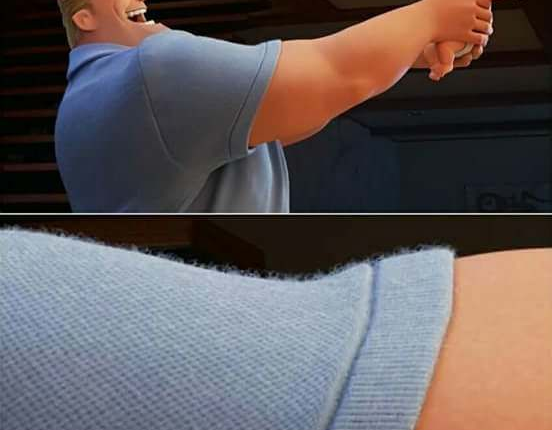
\includegraphics[width=7cm]{incredibles.png}}
\caption{.}
\label{fig:incredibles}
\end{figure}

\section{Background}
\label{sec:background}
Text-to-image generation is made possible through recent advancements in 
Computer Graphics and machine learning.
Two of the most popular concepts applied in the field are generative networks 
using adversarial learning, and attention mechanisms.
Most recently, researchers of text-to-image generation 
have combined both concepts, resulting in new architectures and better ways of 
processing data. In order to provide background for the contributions of each 
paper surveyed herein, an overview of generative adversarial learning and 
attention is provided below.

\subsection{Generative Adversarial Networks}
The Generative Adversarial Network (GAN)
was first proposed as a way to train a network to produce more realistic images
from random noise. The network is made up of two sub-architectures:
a generator, $G$, and a discriminator, $D$. The vanilla GAN model is 
essentially a random image generator, where the generated images share 
qualities of those in the training dataset. A generalization of the basic GAN 
architecture is shown in Figure \ref{fig:gan}.

\begin{figure}[htbp]
\centerline{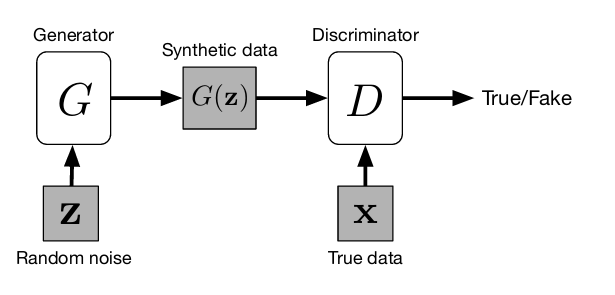
\includegraphics[width=7cm]{gan.png}}
\caption{Basic Generative Adversarial Network architecture, with a 
generator $G$
and discriminator $D$
\cite{cgan}.}
\label{fig:gan}
\end{figure}

The generator is trained to progressively synthesize more realistic images,
while the discriminator is trained to recognize smaller differences between 
real and fake inputs \cite{cgan}. This relationship can be expressed in the 
format of a two-player min-max game, which can be mathematically 
represented as in Equation \ref{eq:gan_basic}.
$p_{data}(\mathbf{x})$ represents the true data distribution,
and $p_{z}(\mathbf{z})$ represents the distribution of noise.

\begin{equation}
\label{eq:gan_basic}
\begin{split}
\text{min}_G\text{max}_DV(D,G) &=
E_{\mathbf{x}\sim p_{data}(\mathbf{x})}[\log D(\mathbf{x})] \\
&+ E_{\mathbf{z}\sim p_{z}(\mathbf{z})}[\log(1 - D(G(\mathbf{z})))]
\end{split}
\end{equation}

Many researchers found it difficult to train the basic GAN model to learn 
global  structures.
While GANs perform excellently as random generative models,
they tend to be unstable,
%are ``\dots notoriously unstable``,
and their outputs often do not reflect the diversity in the training set
\cite{image_transformer}.
%``\dots fail to reflect the diversity in the training set.''
Most recently researchers were able to obtain
higher quality images with more semantic relevance by giving
an algorithm non-random seed data
-- such as a low-quality image or textual description -- to generate from
\cite{texture_synthesis}, \cite{multiscale_video}.
Others found that variation inference and other types of embedding 
increased the quality of generated images \cite{varigan}.
From these discoveries many variant GAN architectures have been produced off of 
the original GAN model.

One such architecture is the Deep Convolutional GAN (DCGAN) was first proposed 
as a way to bridge the capabilities of unsupervised learning  and supervised 
learning (such as Convolutional Neural Networks). 
The DCGAN has a similar structure to the original GAN model, but uses 
convolutional and convolutional-transpose layers in $D$ and $G$, respectively
\cite{unsupervised_learning}. Many frameworks also make use of an image 
enhancement architecture, such as the  Super Resolution GAN (SRGAN) 
\cite{srgan}. The SRGAN takes as input a low-resolution image with possible 
abnormalities, and outputs a larger, higher resolution image with improved 
quality. By combining these techniques and others, researchers created 
architectures such as the MSG-GAN, AttnGAN, and LeicaGAN.

\subsection{Attention Mechanisms}
Attention is a technique that references past data during each iteration of 
training. An attention function a mapping of a query and a
set of key-value pairs to an output \cite{attention_need}.
The mathematical expression of the attention function is shown in
Equation \ref{eq:attention}.
$d_k$ is the dimension of keys and queries, and
$Q,K,V$ are matrices of queries, keys, and values, respectively.
The function uses the dot product operator, so that the output is computed as
a linear combination of weights \cite{attention_need}.

\begin{equation}
\label{eq:attention}
\begin{split}
\text{Attention}(Q,K,V) = \text{softmax}(\frac{QK^T}{\sqrt{d_k}})V
\end{split}
\end{equation}

We can model the joint probability of a sequence,
$\mathbf{x}={x_1,x_2,\dots,x_n}$,
as the product of conditional
probability distributions parameterized by a network $\theta$
\cite{generative_transformers}.
The final expression is shown in Equation \ref{eq:attention_prob}.

\begin{equation}
\label{eq:attention_prob}
p(\mathbf{x}) = \prod_{i=1}^{n}p(x_i|x_1,\dots,x_{i-1};\theta)
\end{equation}

The first proposed attention mechanisms were accomplished by encoding with 
multiple Recurrent Neural Networks (RNNs). However, researchers found this 
strategy lacked efficiency, and created Transformers as
a way to use attention mechanisms more efficiently.
The Transformer relies entirely on self-attention to calculate its 
representations during training, and thus does not require RNNs nor convolution.
%``\dots entirely on self-attention to compute representations of its input and 
%output without using sequence-aligned RNNs or convolution''
\cite{attention_need}.
The encoder and decoder for the Transformer design
are shown in Figure \ref{fig:transformer}.
As demonstrated, an input is first encoded into the dimensional space
the Transformer works with, the network's weights are calculated,
and lastly the result is decoded back as the output of the model.
%The Transformer uses a series of attention functions to map
%between two sequences.
Transformers use a constant number of layers to model an arbitrary number of 
dependencies, which makes them useful for natural language processing and 
image generation \cite{generative_transformers}.

\begin{figure}[htbp]
\centerline{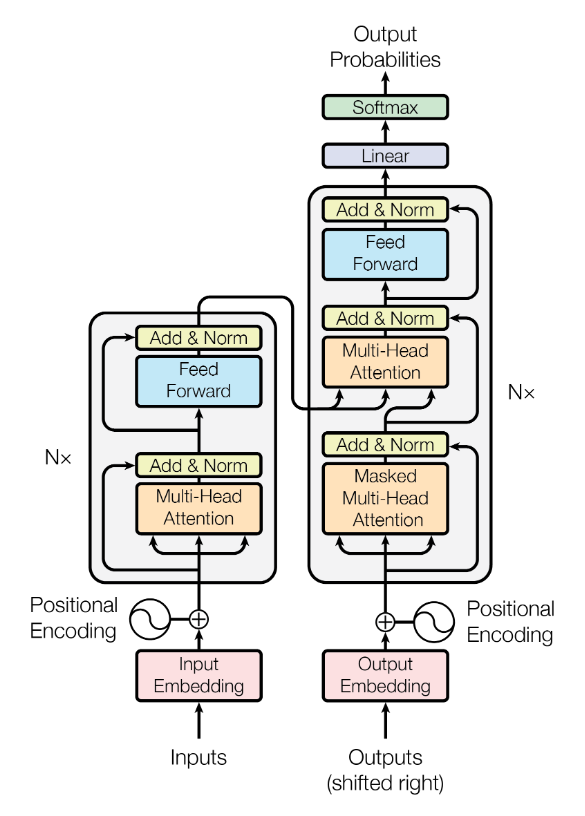
\includegraphics[width=6.5cm]{transformer.png}}
\caption{Transformer architecture showing Encoder and Decoder
\cite{attention_need}.}
\label{fig:transformer}
\end{figure}

%While the Transformer shows potential as a powerful machine learning technique,
%it is a recent concept and still has many inherent problems.
%One of the major problems with the architecture
%is that its required resources scale with $O(n^2)$
%for sequence length $n$.
%Researchers theorize that
%``\dots to improve computational performance for tasks involving very long 
%sequences,
%self-attention could be restricted to considering only a neighborhood of size 
%$r$''
%\cite{attention_need}.
%The Sparse Transformer architecture was developed as a means to shrink the
%computational resources for large sequences of data.
%Child \textit{et al.} introduced sparse factorizations on the attention matrix
%in order to speed up processing \cite{attention_need}.
%They approximated the dense attention
%operation by combining several cheaper attention operations.
%This new method resulted in a faster attention-based architecture
%that could be trained on longer sequences of data 
%\cite{generative_transformers}.
%
%\begin{figure}[htbp]
%\centerline{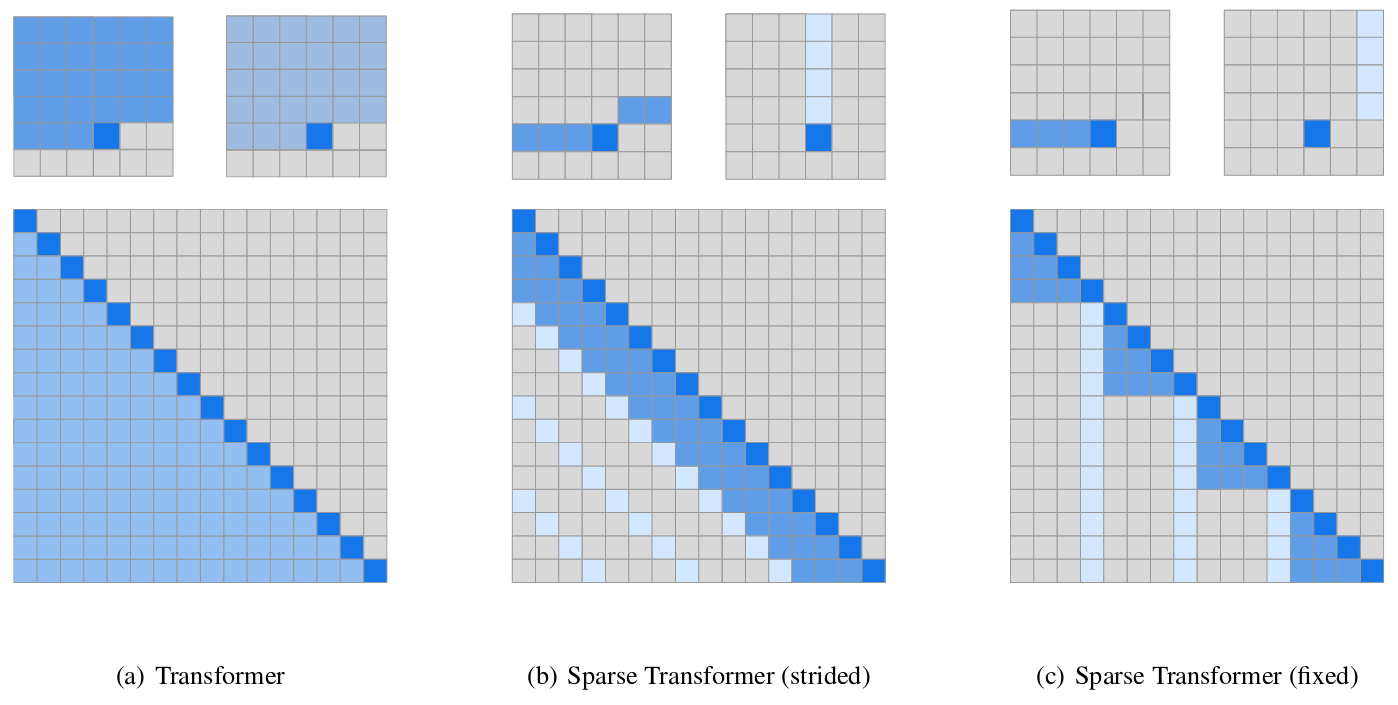
\includegraphics[width=7cm]{sparse_attention.png}}
%\caption{Optimizations of Attention
%\cite{generative_transformers}.}
%\label{fig:attention_optimization}
%\end{figure}
%
%Figure \ref{fig:attention_optimization} shows a visual representation of
%the two optimizations experimented with, strided and fixed.
%The Sparse Attention Transformer architecture
%Sparse attention reduces the resource cost to $O(n\sqrt[p]{n})$.
%The architecture is also simpler than other autoregressive models that perform
%similar functions, including upscaling and enhancement \cite{pixel_subscale}.
%While the Transformer and Sparse Attention Transformer architectures are not 
%directly used in any of the works referenced here, their improvements on 
%attention mechanisms are important to reference as future improvements to the 
%results of our text-to-image generation.

One of the signature contributions of attention, is in learning distinctions 
between components of an image. These distinctions can be represented visually 
in what are called attention maps. An attention map is a black and white weight 
matrix of pixels which shows certainty of an attribute to the image. A dark 
value close to 0 represents no correlation, while lighter values closer to 255 
highlight relevant areas. For example, Figure \ref{fig:attention_example} shows 
the attention maps for a captioning model. The model's output is shown in blue, 
where the important parts are bolded and highlighted by white splotches inside 
the attention maps. Essentially this measures how well the model recognizes the 
meaning of the caption in the input image.

\begin{figure}[htbp]
\centerline{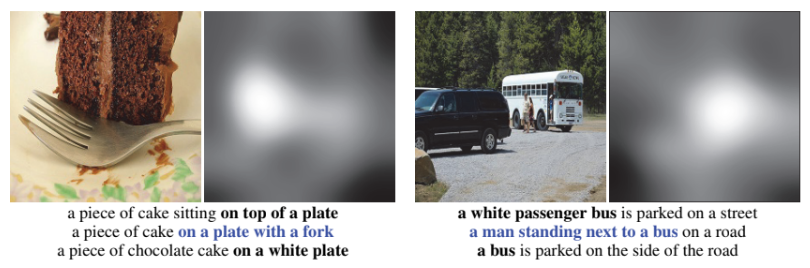
\includegraphics[width=8cm]{attention_example.png}}
\caption{Example of attention maps when applied to image captioning 
\cite{text_captioning}.}
\label{fig:attention_example}
\end{figure}

\section{Related Work}
Although the topic of image generation as a whole is very broad, text-to-image 
generation using machine learning is a newer and lesser studied area. Starting 
as early as 2016 with Reed \textit{et al.}, GANs were applied to image 
generation given textual specifications. Research continues to present day 
where attention mechanisms are being applied as secondary inputs, such as with 
the AttnGAN \cite{attngan} and LeicaGAN \cite{leica} architectures. Here we 
cover some of the most prominent research in the field of text-to-image 
generation, and explain its implications for the future of image synthesis.

%\subsection{Object-driven Text-to-Image Synthesis via Adversarial Training}
%\cite{objgan}

%\subsection{Text-Guided Attention Model for Image Captioning}
%\cite{attention_caption}

\subsection{Generative Adversarial Text to Image Synthesis}
The text-conditional convolutional GAN architecture was one of the first 
GAN architectures to produce success in text-to-image synthesis 
\cite{gan_text_to_image}. To train their generator, data was transmuted into a 
description embedding which they denote as the function $\varphi(t)$. This step 
is  very similar to what is done in many other text-processing machine learning 
models, such as the author's related work on deep representations in image 
classification \cite{deep_visual_descriptions}. Figure \ref{fig:cond_gan} shows 
the GAN architecture developed by Reed \textit{et al.}, which is most similar 
to the DCGAN. Notably, this is the simplest and earliest
architecture of those proposed for this problem. Reed \textit{et al.}
also experimented with the matching-aware discriminator (GAN-CLS) and manifold 
interpolation (GAN-INT) mechanisms. They 
found through testing that a combination of these optimizations gave better 
qualitative results than their base DCGAN model.
The results of their work demonstrate that 
GANs may be stabilized with improved ways of extracting important information 
from unrelated data, which indeed is necessary for the complexity needed in 
text-to-image generation.

\begin{figure}[htbp]
\centerline{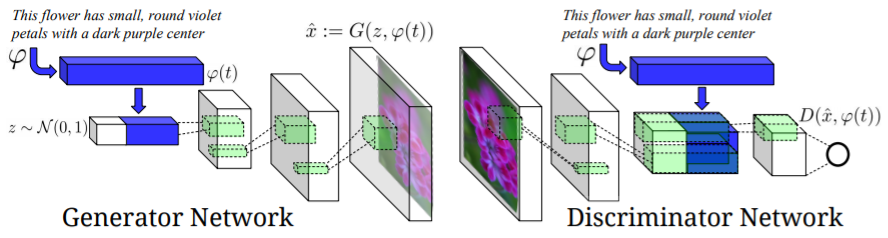
\includegraphics[width=8cm]{cond_gan.png}}
\caption{Text-conditional convolutional GAN architecture, with textual 
description embedding \cite{gan_text_to_image}.}
\label{fig:cond_gan}
\end{figure}

\subsection{AttnGAN: Fine-Grained Text to Image Generation
with Attentional Generative Adversarial Networks}
Text-to-image generation was notably improved by Microsoft Research 
with the advent of the Attentional GAN (AttnGAN) model \cite{attngan}.
Shown in Figure \ref{fig:attngan}, the AttnGAN architecture combines 
inherent inference obtained by the generator and discriminator within the GAN 
framework with the dependency correlation and stability gained from attention 
mechanisms. Instead of encoding the entire sentence as a single input 
vector (e.g. ``this bird has wings that are blue and a red belly``), each word 
in the sentence is allowed an opportunity to claim regional importance in the 
output image. This ability provides better recognition of conditional 
sub-regions, which improves overall semantic relevance of the output image.  
AttnGAN was also based on the work of the StackGAN++ architecture, which found 
a multi-stage approach was necessary for stabilizing sensitivities in training 
GAN models \cite{stackgan++}. Figure \ref{fig:attngan_sample} shows a sample 
input and corresponding output for the AttnGAN model as well as the results of 
attention, demonstrating the semantic relevance of the output image.

\begin{figure}[htbp]
\centerline{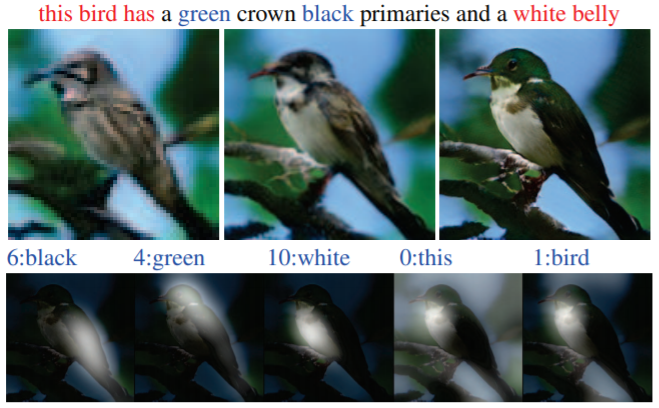
\includegraphics[width=7cm]{attngan_sample.png}}
\caption{Intermediate and final outputs for AttnGAN (top) and the trained 
attention map (bottom)
\cite{attngan}.}
\label{fig:attngan_sample}
\end{figure}

\subsection{MSG-GAN: Multi-Scale Gradients for Generative Adversarial
Networks}
\label{subsec:msg-gan}
The Multi-Scale Gradient GAN (MSG-GAN) was the first GAN to generate images 
with very high resolutions (up to 1024 x 1024 pixels).
Researchers have found it difficult to produce high-resolution images with GANs
``
%This problem is more severe when training GANs to generate
%high-resolution (e.g., 256x256) images
\dots because the chance is
very low for the image distribution and the model distribution
to share supports in a high-dimensional space
'' \cite{stackgan++}.
The MSG-GAN, however, provides mechanisms used by the discriminator to 
reference all resolutions of images generated, which double in size starting as 
small as 4 x 4. By referencing the outputs of all intermediate layers, the 
MSG-GAN acquires more stability during training, and thus produces better 
outputs for all generated resolutions
%``
%MSG-GAN allows
%the discriminator to look at not only the final output (highest resolution) of 
%the generator, but also at the outputs of
%the intermediate layers 
%''
\cite{msggan}. Figure \ref{fig:msggan} shows results of the MSG-GAN generating 
very small (left) and very high (right) resolutions for a given input.
Their approach will undoubtedly revolutionize how we generate images in the 
future, especially for high-resolution outputs such as rendered frames.

\begin{figure}[htbp]
\centerline{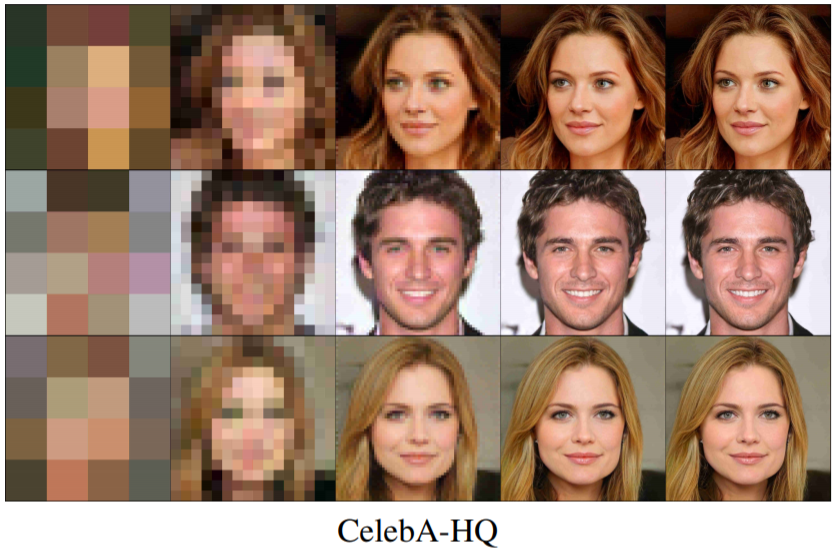
\includegraphics[width=7cm]{msggan.png}}
\caption{MSG-GAN results for increasing resolutions
\cite{msggan}.}
\label{fig:msggan}
\end{figure}

\subsection{Learn, Imagine and Create: Text-to-Image Generation from Prior 
Knowledge}
\label{subsec:leica}
A new architecture was created from the advancements of AttnGAN, called LEarn, 
Imagine and CreAte GAN (LeicaGAN) \cite{leica}. Similar to other 
attention-based GANs, the LeicaGAN architecture is comprised of a 
text-embedding phase, followed by coarse-to-fine image generators. The main 
difference in the LeicaGAN is their use of textual-visual co-embedding (TVE) 
and multiple priors aggregation (MPA) to further extract semantic meaning from 
their inputs. The authors argue that their architecture more closely models how 
the human brain analyzes textual data, and therefore will have better results 
in identifying the relationships between an image and its textual description.

\begin{figure}[htbp]
\centerline{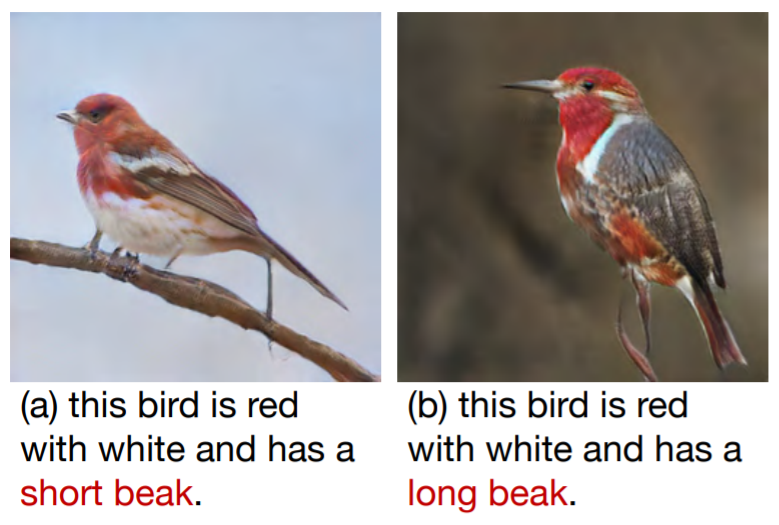
\includegraphics[width=7cm]{leicagan_sample.png}}
\caption{Image outputs of LeicaGAN for similar input sentences
\cite{leica}.}
\label{fig:leica_sample}
\end{figure}

Figure \ref{fig:leica_sample} demonstrates how images may differ from changing 
one attribute only. A by-product of this change is that the setting and pose 
are completely different. Further analysis is needed to determine how much of 
this can be controlled analytically. Figure \ref{fig:leicagan} shows the 
results of LeicaGAN on the CUB bird and Oxford-102 flower datasets, as well as 
results of AttnGAN for comparison. Their analysis shows that LeicaGAN is 
objectively better than previous state-of-the-art methods for text-to-image 
generation.

\section{Term Work}
Many architectures could be applied to image and text processing. Our focus was 
to identify possible candidates which could be used effectively for 
text-to-image generation, and in what ways. Although the LeicaGAN architecture 
achieved the best results out of all models 
surveyed, the network proved too complex to incorporate it into a working 
pipeline. The AttnGAN model, which is a few years older than LeicaGAN, was 
evaluated instead. We found AttnGAN to produce remarkable results, which are 
discussed in further detail in Section \ref{subsec:results}.

\subsection{Architecture}
The AttnGAN architecture, shown in Figure \ref{fig:attngan}, trains several 
types of embedded sub-architectures. Attention mechanisms and Generative 
Adversarial Networks (GANs) were covered in Section \ref{sec:background}, so we 
will focus on the other architectures used to create the impressive results of 
AttnGAN.

Image processing often uses Convolutional Neural Networks (CNNs), which excel 
in feature extraction from images. As discussed previously, GANs are currently 
the most popular image generators and are widely used in image synthesis or 
modification. The Recurrent Neural Network (RNN) 
excels in sequence-to-sequence learning, such as natural language processing or 
language translation. The network was found to handle temporal data very well, 
but failed when the data experienced permutations or when relationships spanned 
several nodes. To help solve this, the Long Short-Term Memory (LSTM) network 
was created, which is similar to the RNN but contains several feedback pathways 
which help facilitate learning the relationships of longer sequences.
AttnGAN uses a combination of attention mechanisms and GAN models for image 
generation, and combines the CNN and LSTM architectures for text and image 
embedding.

\begin{figure}[htbp]
\centerline{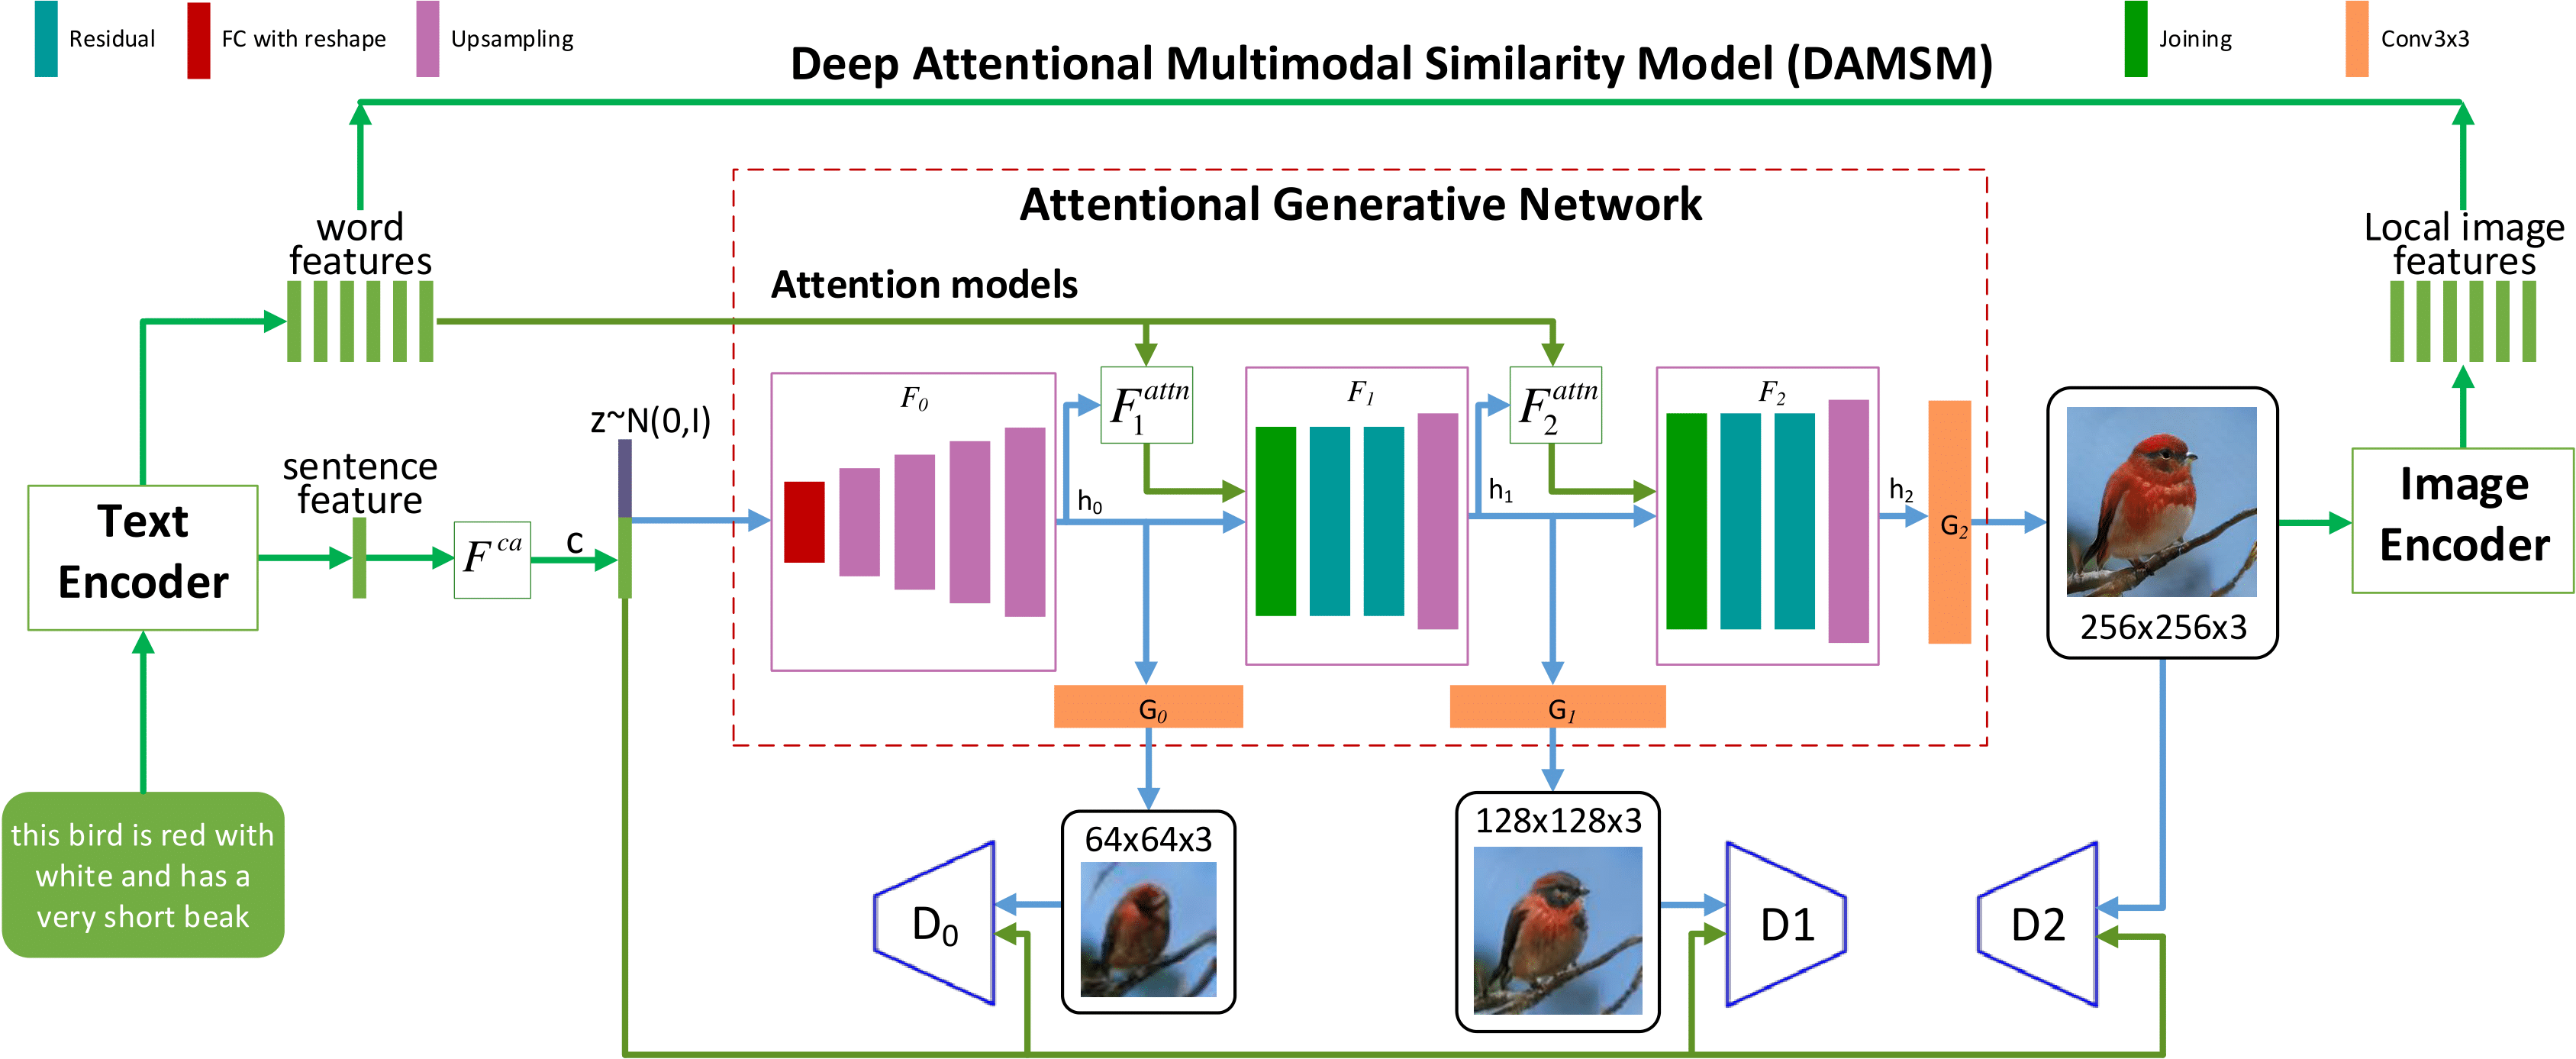
\includegraphics[width=8cm]{attngan.png}}
\caption{AttnGAN architecture, showing separate generators and introduction 
of Attention mechanisms.}
\label{fig:attngan}
\end{figure}

\subsection{Process}
The final process developed for this term is shown by the flow diagram in 
Figure \ref{fig:flow_diagram}. As shown, the pipeline in its un-optimized state 
is very costly both in computational resources and time. A majority of the time 
spent in the pipeline is in the model training stages, which account for 24 
hours of total processing time. Less expensive stages of the pipeline include 
pre-processing network inputs as well as evaluating end results.

We begin our process by generating training data.
This data must be generated for each frame of the animation, and similarly 
processed by the animation software in order to generate the pair of 
information which constitutes an input block. An input frame is processed in 
order to create a dataset with minimal similarity between two elements. This 
helps curb overtraining for background blocks which show little 
to no changes throughout the animation.

The small blocks of each frame (referred to herein as ``frameblocks'') and the 
text data which helps identify them are generated in separate pre-processing 
stages of the pipeline. Our input animation of 120 frames 
generated a total of over 34,000 frameblocks of size 64 x 64 pixes. These were 
exported and stored in the dataset to be used in training.
Attributes are generated from scene data for each possible frameblock of every 
frame. For our small-sized scene, processing all 120 frame took approximately 
10 hours to complete. After all attribute files are generated, they are 
matched to their corresponding frameblocks to create the input pair into the 
machine learning architecture.

\begin{figure}[htbp]
\centerline{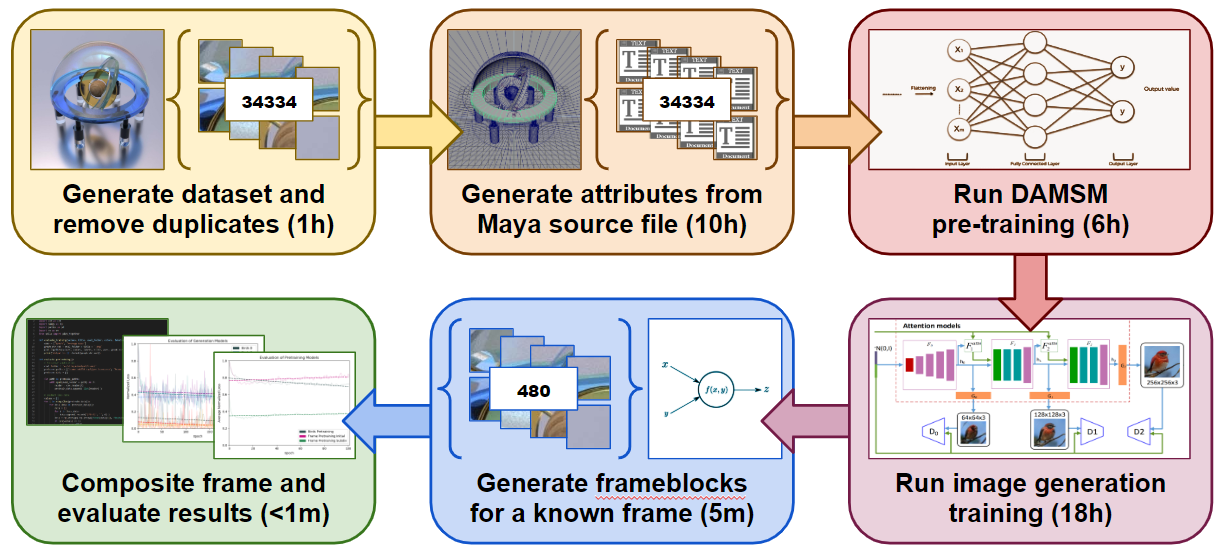
\includegraphics[width=8.5cm]{flow_diagram.png}}
\caption{Flow diagram for the process of the entire developed network.}
\label{fig:flow_diagram}
\end{figure}

\subsection{Training}
The Caltech-UCSD Birds-200-2011 (CUBS) dataset was used for initial training of 
the AttnGAN network \cite{cubs}. CUBS contains 200 categories of bird types 
with a total of 11,788 images. The attribute data is contained in multiple 
variable-length captions for each image. Here the term ``caption'' refers to 
characteristics of what is shown in the image. An example caption from CUBS is 
``this bird has a bright yellow crown, a long straight bill, and white 
wingbars.''. Before training begins, the architecture reads in all captions and 
creates a one-hot encoding on each word, meaning each word is assigned a bit 
value of a binary string of size $n$, where $n$ is the total number of 
captions. This creates an easy way for the network to recognize words and 
ensures words remain distinct from one another.

We first trained on the CUBS dataset in order to provide a baseline for 
comparison. After obtaining feasible results from CUBS, we generated worked on 
generating images from our dataset of frameblocks. The evolution of results for 
both datasets during training are shown in 
Figure \ref{fig:evolution}, where $\mathbf{e}$ represents the training epoch. 
An epoch refers to one iteration through the entire dataset. Thus the CUBS 
dataset looks at around 10,000 elements, and our frame dataset looks at over 
13,000. Total epochs were capped at 250 for evaluation purposes, however in 
practice the architecture would be allowed to train until loss stabilized.

\begin{figure}[h!]
\centering
\begin{subfigure}{0.22\textwidth}
\begin{center}
\begin{minipage}[t]{0.95\linewidth}
\begin{centering}
% BIRDS
{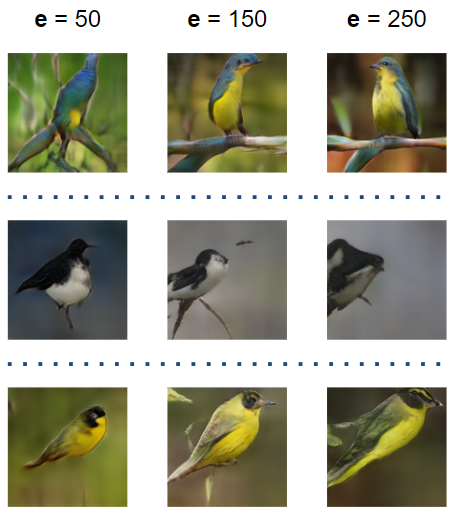
\includegraphics[width=\linewidth]{evolution_birds.png}}
\caption{Samples for CUBS.}
\label{fig:evolution_birds}
\end{centering}
\end{minipage}
\end{center}
\end{subfigure}
\begin{subfigure}{0.22\textwidth}
\begin{center}
\begin{minipage}[t]{0.95\linewidth}
\begin{centering}
% FRAME
{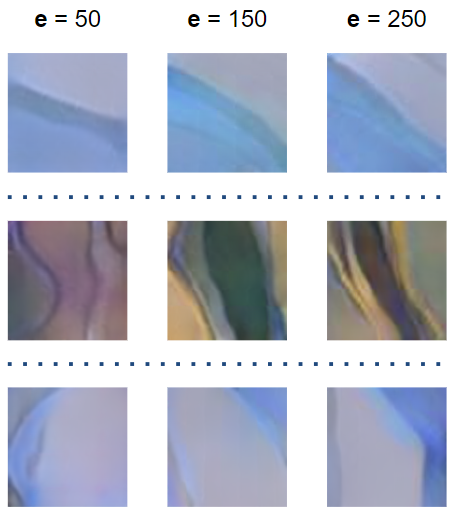
\includegraphics[width=\linewidth]{evolution_frame.png}}
\caption{Samples for frames.}
\label{fig:evolution_frame}
\end{centering}
\end{minipage}
\end{center}
\end{subfigure}
\caption{Evolution of an input during training, showing results at 50, 150, and 
250 epochs for 3 samples of each dataset.}
\label{fig:evolution}
\end{figure}

All 480 attributes for a sample frame were fed into the trained model, which 
generated 480 frameblocks. The reconstructed frame is shown in Figure 
\ref{fig:initial_full} , adjacent to the target sample. While our initial 
result has general shape and detail, there are clearly many problems.
The background blocks have appropriate lighting, however they do not have 
enough cross-boundary coherence. This is consistent with the rest of the blocks 
of the sample, where the problem is exacerbated by anomalies. Some blocks 
appear randomly placed, although the more prevalent problem is in representing 
multiple objects within one block. The architecture has not learned how to 
represent the boundaries between objects, which causes a kaleidoscope effect 
for the generated frame as a whole.
Another major issue is in generating opposite sides of symmetric objects. The 
architecture learned to generate only one side of the object, which leads to a 
misalignment of the frameblocks within the image. It was also common for 
over-training to occur on portions of most objects, such that a pattern 
found in one block was replicated to other similar blocks.

\subsection{Improvements}
\begin{figure}[htbp]
\centerline{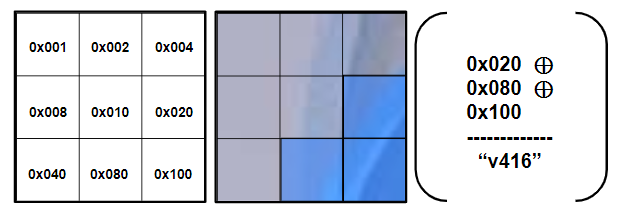
\includegraphics[width=8cm]{subdivision.png}}
\caption{Example of precision being added to initial architecture.}
\label{fig:subdivision}
\end{figure}

\subsection{Final Results}
\label{subsec:results}

\subsection{Evaluation Criteria}
A major criticism of GANs and other generative models is that no robust 
evaluation methods exist.
As opposed to other machine learning models, GANs do not optimize any kind of 
objective function,
and operate instead on a learned latent space
which cannot be analyzed analytically \cite{gmm}.
Thus, in order to evaluate the implemented models,
we must find a way to numerically compare the generated images to their 
respective targets.

%Researchers have defined many different means of comparing two images.
%Some of this research is focused on image context, such as if two images 
%contain the same
%person or setting.
%This type of analysis would not benefit our project,
%since the image needs to be exact --
%simply containing similar features is not enough.
%Thus, we turned to the measurements of
%Mean Squared Error (MSE) and Peak Signal-To-Noise Ratio (PSNR),
%as both metrics are commonly used to evaluate super resolution algorithms
%\cite{super_resolution}.
%
%``
%Inception Score and R-precision are regarded as effective and are commonly 
%used 
%for evaluating the diversity of the generated images \dots it was observed 
%that 
%a
%text-to-image model could get a fairly high performance even when the model 
%actually generated
%visually-low quality images
%''
%\cite{leica}.

Since the generated birds from CUBS do not match one-to-one as our frame data 
does, we decided loss measurements were appropriate for comparing the two 
datasets. These results are 
We plan to use methods such as Mean Squared Error (MSE) and Peak 
Signal-To-Noise Ratio (PSNR) to compare images for other datasets we'll test in 
the future \cite{srgan}. One such dataset is Visual Genome, which is a large 
database with a total of 108,077 images and millions of registered attributes 
\cite{visual_genome}. Some of our work involved extracting custom attributes 
for each frameblock from Visual Genome to be used later as more useful 
comparison to results from our dataset. An example of our feature extraction 
work for Visual Genome is shown in Figure \ref{fig:visual_genome}. We hope to 
exploit the massive amounts of descriptive data from Visual Genome's 2D scenes 
to improve generating images for 3D frame data.

\begin{figure}[htbp]
\centerline{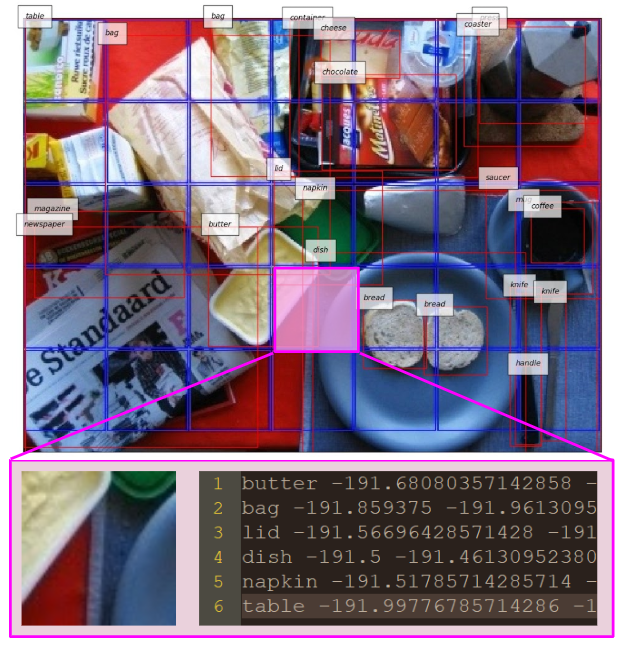
\includegraphics[width=7cm]{visual_genome.png}}
\caption{Block and attribute extraction for a sample of the Visual Genome 
dataset.}
\label{fig:visual_genome}
\end{figure}

Loss measurements for the AttnGAN architecture are shown by the graphs in 
Figure \ref{fig:loss}. Training the encoders (pretraining) and generative 
training losses were graphed separately, since they had differing loss 
measurements. Each graph contains losses for all models trained, including 
CUBS, initial frame, and improved frame. We found that the attributes 
themselves caused variation in training the 
DAMSM and generation models between the CUBS dataset and ours. Specifically, 
the higher-precision frame model performed approximately 119\% better than the 
original model, and significantly improved on the CUBS baseline. We theorize 
that this is because the added precision enabled the text and image encoders to 
more effectively identify portions of the images, which is exactly the 
effect we had hoped for.

Compared to pretraining, loss only improved by around 6\% for the generative 
models, and the CUBS and frame datasets were very close in loss. This means 
that the added precision was not as reflected in generated frameblocks. 
Analyzing the results further, we found that while the details of each block 
were generally better, the structure did not improve. Figure 
\ref{fig:final_comp}.

\begin{figure}[h!]
\centering
\begin{subfigure}{0.5\textwidth}
\begin{center}
\begin{minipage}[t]{0.95\linewidth}
\begin{centering}
% BIRDS
{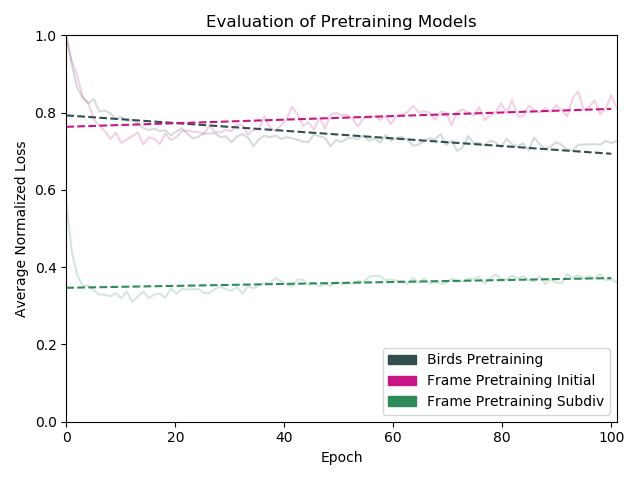
\includegraphics[width=\linewidth]{eval_pretrain.png}}
\caption{Loss measurements during pretraining DAMSM model.}
\label{fig:eval_pretrain}
\end{centering}
\end{minipage}
\end{center}
\end{subfigure}
\par\medskip
\begin{subfigure}{0.5\textwidth}
\begin{center}
\begin{minipage}[t]{0.95\linewidth}
\begin{centering}
% FRAME
{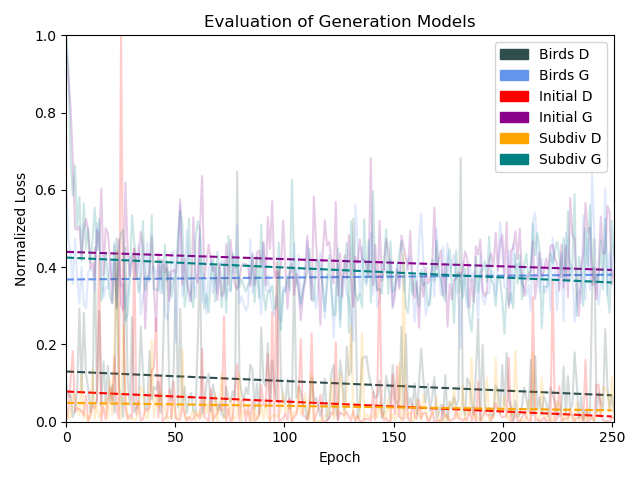
\includegraphics[width=\linewidth]{eval_gentrain.png}}
\caption{Loss measurements during training generative models.}
\label{fig:eval_gentrain}
\end{centering}
\end{minipage}
\end{center}
\end{subfigure}
\caption{Evaluation of training loss for AttnGAN models.}
\label{fig:loss}
\end{figure}

Yet another method we can use to analyze the AttnGAN architecture is by 
analyzing the generated attention maps for a given sample of each dataset. 
Figure \ref{fig:final_comp} shows attention maps for generated blocks and their 
corresponding input attributes.

\begin{figure}[htbp]
\centerline{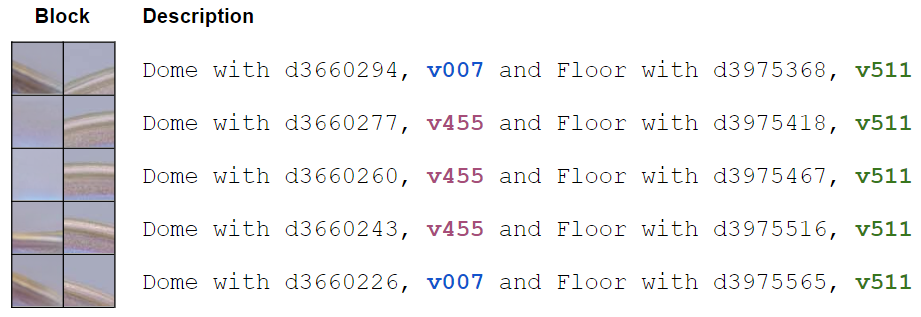
\includegraphics[width=8.5cm]{final_comp.png}}
\caption{Analysis of some problematic blocks in the final output.}
\label{fig:final_comp}
\end{figure}

\begin{figure}[h!]
\centering
\begin{subfigure}{0.5\textwidth}
\begin{center}
\begin{minipage}[t]{0.95\linewidth}
\begin{centering}
% BIRDS
{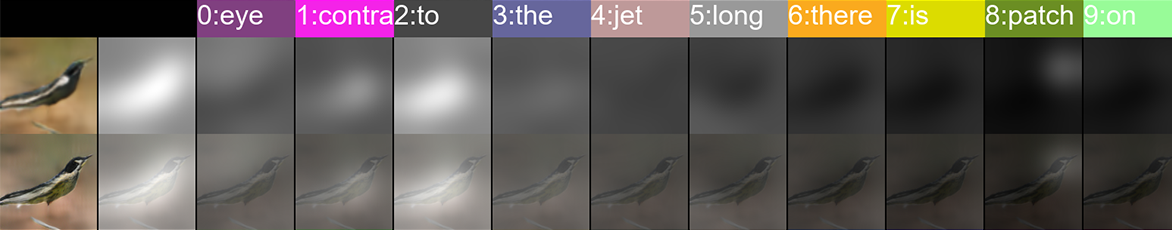
\includegraphics[width=\linewidth]{maps_birds.png}}
\caption{Attention maps for a sample from CUBS dataset.}
\label{fig:maps_birds}
\end{centering}
\end{minipage}
\end{center}
\end{subfigure}
\par\medskip
\begin{subfigure}{0.5\textwidth}
\begin{center}
\begin{minipage}[t]{0.95\linewidth}
\begin{centering}
% FRAME
{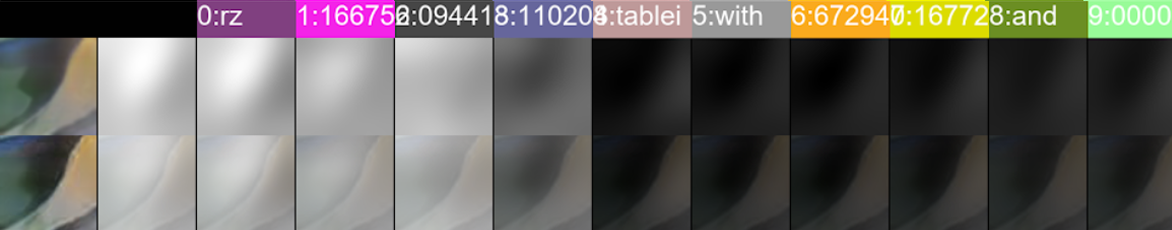
\includegraphics[width=\linewidth]{maps_frame.png}}
\caption{Attention maps for a sample of our frame dataset.}
\label{fig:maps_frame}
\end{centering}
\end{minipage}
\end{center}
\end{subfigure}
\caption{Evaluation of attention mechanisms for input attributes of each 
dataset.}
\label{fig:maps}
\end{figure}

\section{Future Work}
The success of our study show the potential for text-to-image generation and 
its applications to deep rendering. Our results are still very crude, however, 
and require further optimization and refinement. We plan to add more precision 
to our current model, by compiling more unique scene data into the input 
attributes.

\begin{figure}[htbp]
\centerline{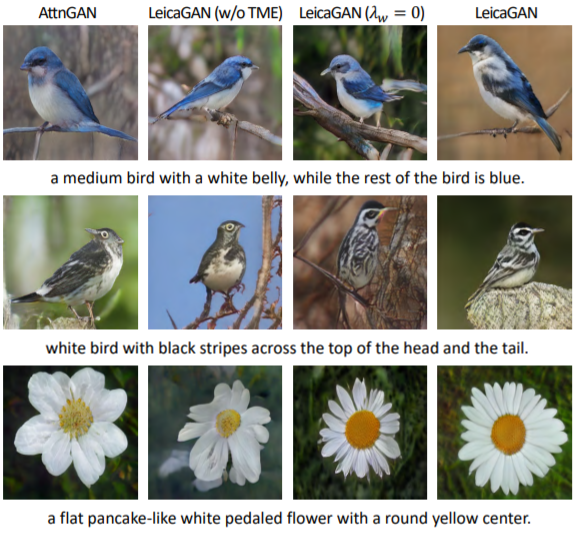
\includegraphics[width=7.75cm]{leicagan.png}}
\caption{LeicaGAN results with varied hyperparameters (right columns), compared 
to results 
of AttnGAN (left column)\cite{leica}.}
\label{fig:leicagan}
\end{figure}

It may still be possible to work with our poor results through the use of a 
post-processing clean up phase. One such method is the use of a super 
resolution network, such as the SRGAN \cite{srgan}. We were able to use this 
network in particular to remove anomalies of varying degrees from input images. 
An example of this process is shown in Figure \ref{fig:srgan}. Both noise 
($\alpha$) and blur ($\beta$) were varied in order to obtain datasets with 
random distributes of anomalies. The results of SRGAN show the potential for 
removing anomalous blocks from those generated.

\begin{figure}[htbp]
\centerline{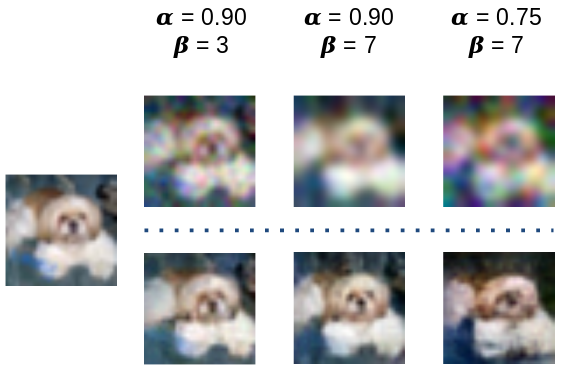
\includegraphics[width=8cm]{srgan_outputs.png}}
\caption{Experimental outputs of SRGAN model for varying noise ($\alpha$) and 
blur ($\beta$) parameters.}
\label{fig:srgan}
\end{figure}

It is unlikely that the SRGAN will work well without first improving the global 
structure of generated frames. For this reason we also propose the use of the 
MSG-GAN, discussed in Section \ref{subsec:msg-gan}. As Figure 
\ref{fig:subdiv_avg} shows, the downsampled version of our output is fairly 
close to the downsampled version of the target frame. It may be possible to 
train the MSG-GAN to upsample from such input, in order to produce the full 
resolution quality (1920 x 1080). We will look into the implications of this 
idea and explore possible optimizations for training and the proposed 
post-processing steps.

\section{Conclusion}
\label{sec:conclusion}
Since the dawn of humanity, manually creating images through drawing, 
painting, or rendering has been the only available method for image generation. 
However the recent application of complex artificial neural networks
has broken through the creative glass ceiling, and opened the door to new image 
generation prospects. With the advent of Generative Adversarial Networks, we 
now have models capable of generating images. Since many researchers found that 
conditional GANs easily become unstable and at times generate 
undesired results, they are now utilizing the concept of 
attention to synthesize higher-quality images with more semantic relevance. 
%The AttnGAN and LeicaGAN architectures are both excellent examples of mature 
%text-to-image generation models.
Using the AttnGAN created by Microsoft Research, we successfully created a 
proof of concept for generating a frame of animation without a renderer. We 
look forward to seeing the application of these models to context-aware image 
generation, as well as other difficult problems in the field of Computer 
Graphics and Computer Vision.

\nocite{objgan}
\nocite{mirrorgan}

\bibliography{final}
\bibliographystyle{aaai}

\begin{figure*}[h!]
\centering
\begin{subfigure}{\textwidth}
\begin{center}
\begin{minipage}[t]{0.95\linewidth}
\begin{centering}
% INITIAL
{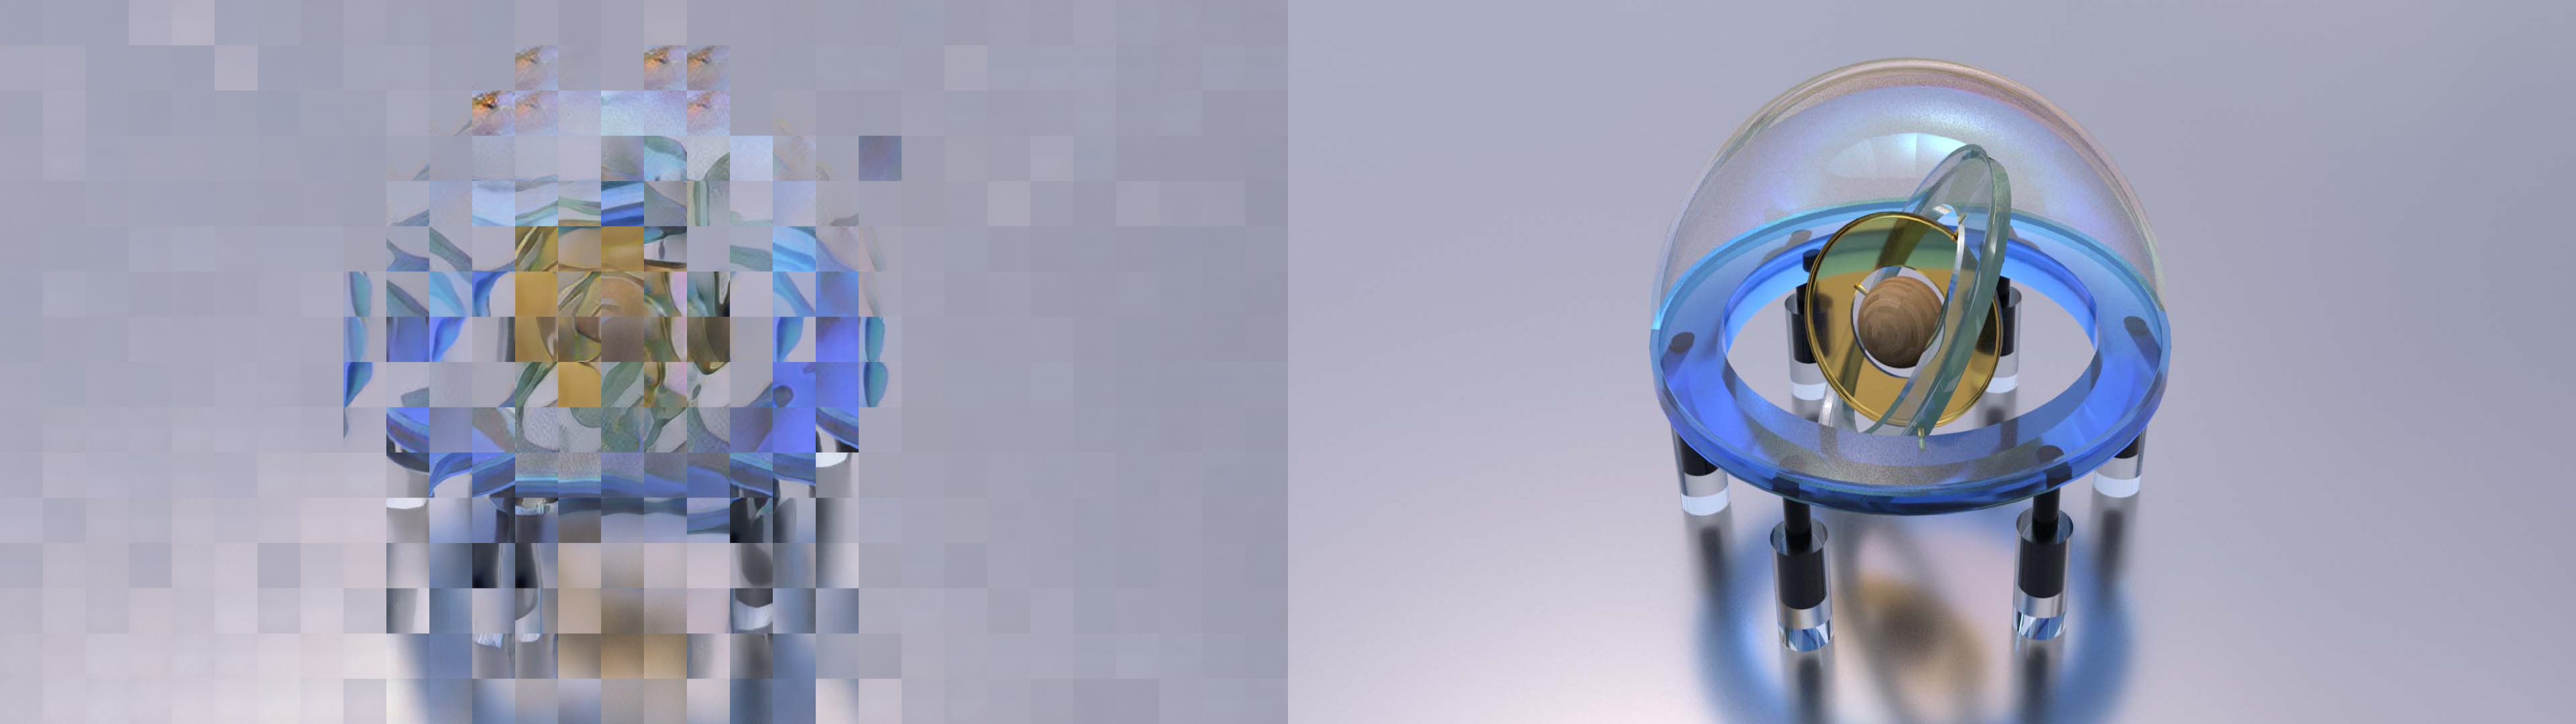
\includegraphics[width=\linewidth]{initial_full.png}}
\caption{Initial generated frame (left), compared to target at full resolution 
(right).}
\label{fig:initial_full}
\end{centering}
\end{minipage}
\end{center}
\end{subfigure}
\par\bigskip
\begin{subfigure}{\textwidth}
\begin{center}
\begin{minipage}[t]{0.95\linewidth}
\begin{centering}
% FINAL
{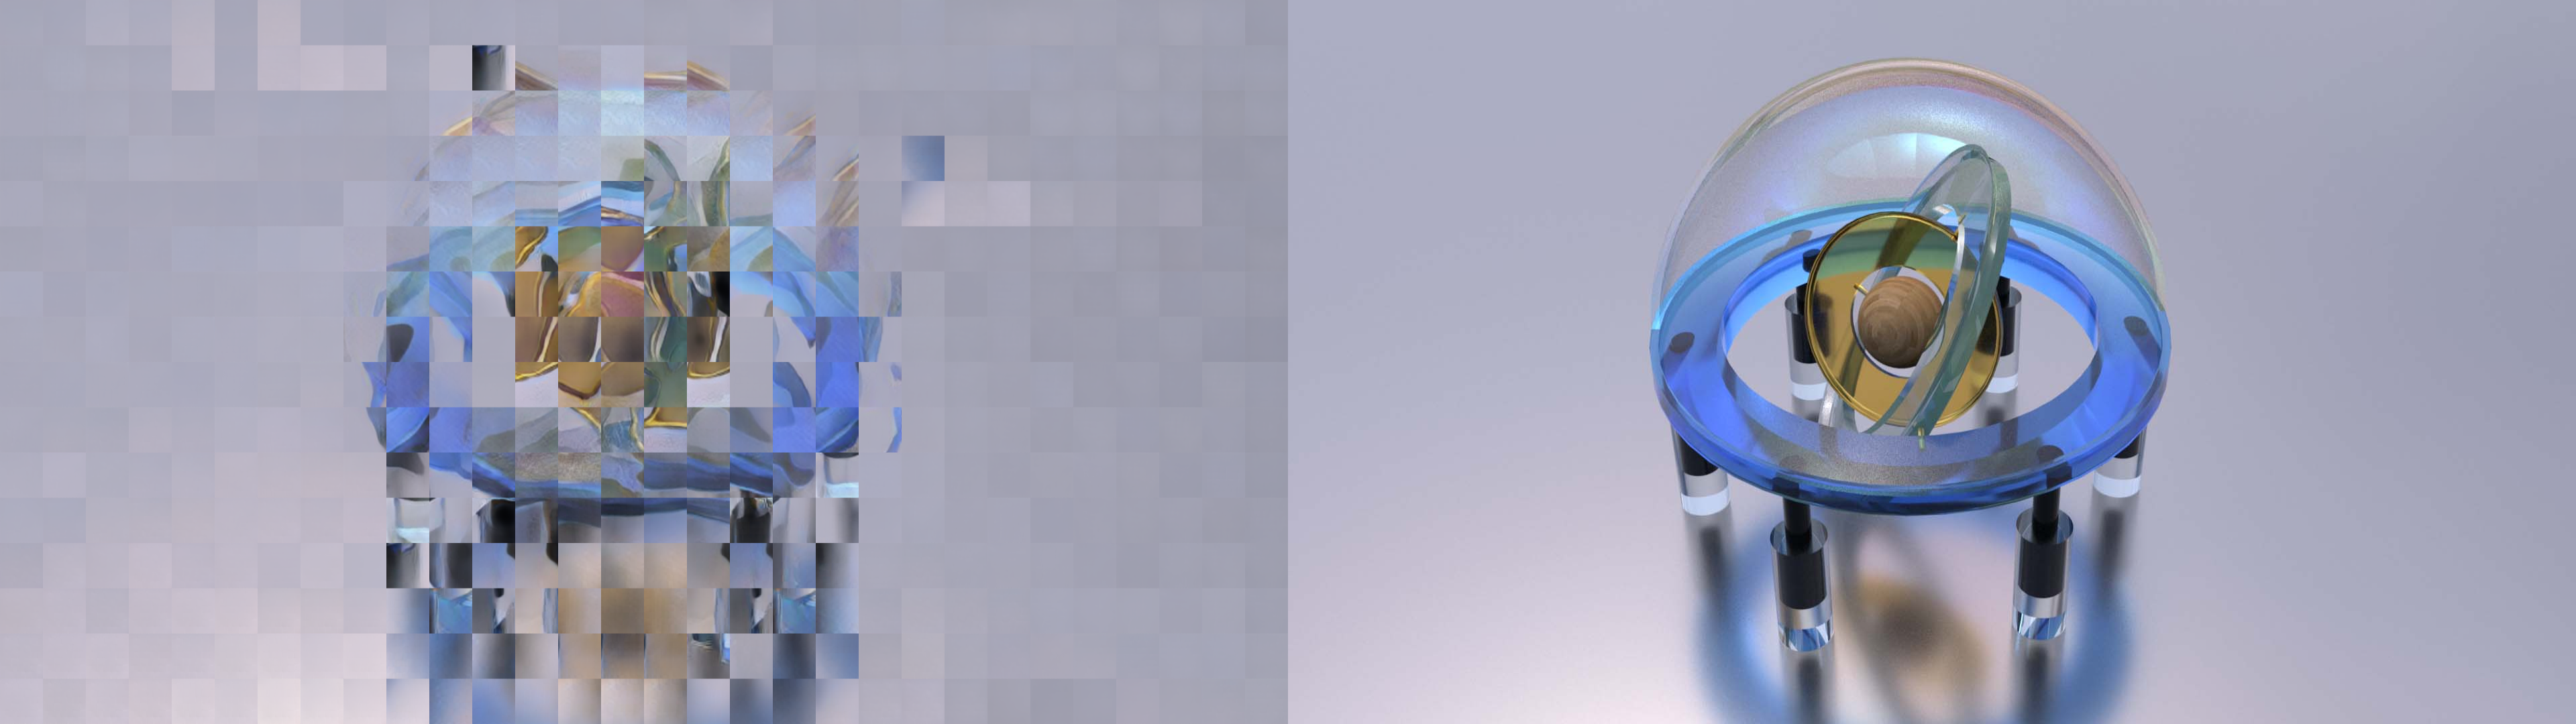
\includegraphics[width=\linewidth]{subdiv_full.png}}
\caption{Final generated frame (left), compared to target at full resolution 
(right).}
\label{fig:subdiv_full}
\end{centering}
\end{minipage}
\end{center}
\end{subfigure}
\par\bigskip
\begin{subfigure}{\textwidth}
\begin{center}
\begin{minipage}[t]{0.95\linewidth}
\begin{centering}
% AVG
{
\includegraphics[width=\linewidth]{subdiv_avg.png}}
\caption{Average value for each block of final frame (left), compared to target 
at 
matching resolution (right).}
\label{fig:subdiv_avg}
\end{centering}
\end{minipage}
\end{center}
\end{subfigure}
\caption{Results for frame generation using adapted network architecture.}
\label{fig:results}
\end{figure*}

\end{document}
